\question
A function $f$ is continuous, differentiable, and strictly decreasing on the interval $[2.5,5]$; 
some values of $f$ are shown in the table below.
\begin{center}
  \begin{tabular}{c|cccccc}
  $x$ & 2.5 & 3.2 & 3.5 & 4.0 & 4.6 & 5.0 \\
  \hline
  $f(x)$ & 7.6 & 5.7 & 4.2 & 3.1 & 2.2 & 1.5 \\
  \end{tabular}
\end{center}
\begin{enumerate}
\renewcommand{\labelenumi}{(\alph{enumi})}
\item Estimate $f^{\prime}(4.0)$ and $f^{\prime}(4.8)$.
\begin{solutionorbox}[1.5in]
$f^{\prime}(4.0) \simeq \dfrac{f(4.6)-f(4.0)}{4.6-4.0}=\dfrac{2.2-3.1}{0.6}=-1.5$.
\[
f^{\prime}(4.8) \simeq \dfrac{f(5)-f(4.6)}{5-4.6}=\dfrac{1.5-2.2}{0.4}=-1.75 .
\]
\end{solutionorbox}

\item What does the table suggest may be true of the concavity of $f$? Explain.
\begin{solutionorbox}[1in]
It appears that the rate of change of $f$, while negative, is increasing. This implies that the graph of $f$ is concave upward.
\end{solutionorbox}

\item Estimate $\int_{2.5}^{5} f(x) d x$ with a Riemann sum using left endpoints.
\begin{solutionorbox}[1in]
$L=7.6(0.7)+5.7(0.3)+4.2(0.5)+3.1(0.6)+2.2(0.4)=11.87$.
\end{solutionorbox}

\item Set up (but do not evaluate) a Riemann sum that estimates the volume of the solid formed when $f$ is rotated around the $x$-axis.
\begin{solutionorbox}[1.5in]
Using disks $\Delta V=\pi r^{2} \Delta x$. One possible answer uses the left endpoints of the subintervals as values of $r$ :
\[
V \approx \pi(7.6)^{2}(0.7)+\pi(5.7)^{2}(0.3)+\pi(4.2)^{2}(0.5)+\pi(3.1)^{2}(0.6)+\pi(2.2)^{2}(0.4)
\]
\end{solutionorbox}
\end{enumerate}


\newpage

\question
The equation of the tangent line to the curve $x^{2} y-x=y^{3}-8$ at the point $(0,2)$ is $12 y+x=24$.

\begin{enumerate}
\renewcommand{\labelenumi}{(\alph{enumi})}
\item Given that the point $\left(0.3, y_{0}\right)$ is on the curve, find $y_{0}$ approximately, using the tangent line.
\begin{solutionorbox}[1in]
$12 y_{0}+0.3=24$ yields $y_{0} \simeq 1.975$.
\end{solutionorbox}

\item Find the true value of $y_{0}$.
\begin{solutionorbox}[2in]
Replace $x$ by 0.3 in the equation of the curve:

\[
\begin{gathered}
(0.3)^{2} y_{0}-(0.3)=y_{0}^{3}-8 \text { or } \\
y_{0}^{3}-0.09 y_{0}-7.7=0
\end{gathered}
\]

The calculator's solution to three decimal places is $y_{0}=1.990$.
\end{solutionorbox}

\item What can you conclude about the curve near $x=0$ from your answers to parts (a) and (b)?
\begin{solutionorbox}[1.5in]
Since the true value of $y_{0}$ at $x=0.3$ exceeds the approximation, conclude that the given curve is concave up near $x=0$. (Therefore, it is above the line tangent at $x=0$.)
\end{solutionorbox}
\end{enumerate}




\newpage






\question
Draw a graph of $y=f(x)$, given that $f$ satisfies all the following conditions:

\statementbox{%
\begin{enumerate}
\renewcommand{\labelenumi}{(\arabic{enumi})}
\item $f^{\prime}(-1)=f^{\prime}(1)=0$.
\item If $x<-1$, $f^{\prime}(x)>0$ but $f^{\prime \prime}<0$.
\item If $-1<x<0$, $f^{\prime}(x)>0$ and $f^{\prime \prime}>0$.
\item If $0<x<1$, $f^{\prime}(x)>0$ but $f^{\prime \prime}<0$.
\item If $x>1$, $f^{\prime}(x)<0$ and $f^{\prime \prime}<0$.
\end{enumerate}%
}
\begin{solutionorbox}[2.5in]
The graph shown below satisfies all five conditions. So do many others!\\
\begin{center}
  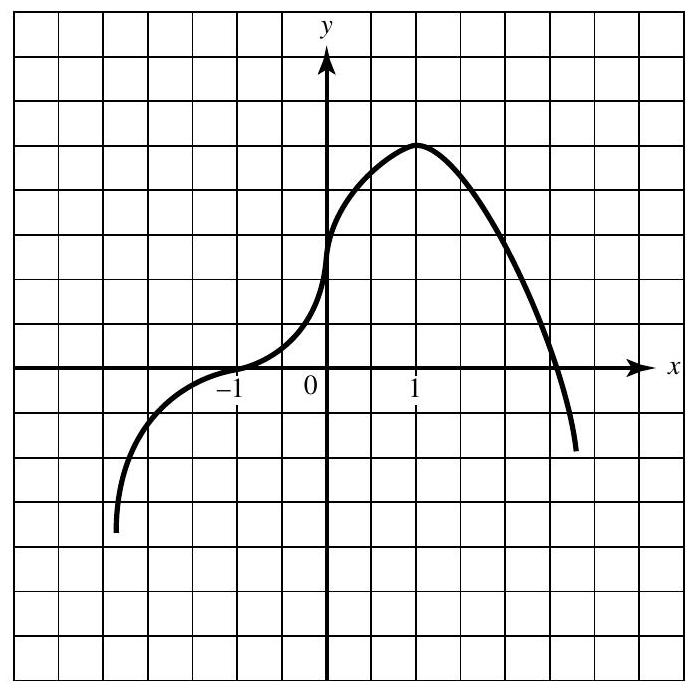
\includegraphics[width=0.70\linewidth]{calculus/images/71c445d1-6f5c-451e-be73-f2e2b89ae7db-07_690_697_1774_674.jpg}
\end{center}
\end{solutionorbox}



\newpage




\question
A differentiable function $f$ defined on $-7<x<7$ has $f(0)=0$ and $f^{\prime}(x)= 2 x \sin x-e^{-x^{2}}+1$. (Note: The following questions refer to $f$, not to $f^{\prime}$.)



\begin{enumerate}
\renewcommand{\labelenumi}{(\alph{enumi})}
\item Describe the symmetry of $f$.
\begin{solutionorbox}[1in]
  Graph $f^{\prime}(x)=2 x \sin x-e^{\left(-x^{2}\right)}+1$ in $[-7,7] \times[-10,10]$.\\
  \begin{center}
    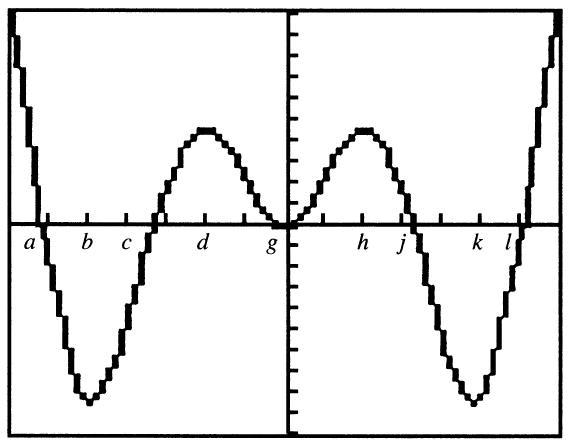
\includegraphics[width=0.40\linewidth]{calculus/images/71c445d1-6f5c-451e-be73-f2e2b89ae7db-08_446_570_392_1080.jpg}
  \end{center}
  Since $f^{\prime}$ is even and $f$ contains ( 0,0 ), $f$ is odd and its graph is symmetric about the origin.
\end{solutionorbox}

\item On what intervals is $f$ decreasing?
\begin{solutionorbox}[1.5in]
Since $f$ is decreasing when $f^{\prime}<0, f$ decreases on the intervals ( $a, c$ ) and $(j, l)$. Use the calculator to solve $f^{\prime}(x)=0$. Conclude that $f$ decreases on $-6.202<x<-3.294$ and (symmetrically) on $3.294<x<6.202$.
\end{solutionorbox}

\item For what values of $x$ does $f$ have a relative maximum? Justify your answer.
\begin{solutionorbox}[1.5in]
$f$ has a relative maximum at $x=q$ if $f^{\prime}(q)=0$ and if $f$ changes from increasing $\left(f^{\prime}>0\right)$ to decreasing $\left(f^{\prime}<0\right)$ at $q$. There are two relative maxima here: at $x=a=-6.202$ and at $x=j=3.294$.
\end{solutionorbox}

\item How many points of inflection does $f$ have? Justify your answer.
\begin{solutionorbox}[1.5in]
$f$ has a point of inflection when the graph of $f$ changes its concavity; that is, when $f^{\prime}$ changes from increasing to decreasing, as it does at points $d$ and $h$, or when $f$ changes from decreasing to increasing, as it does at points $b, g$, and $k$. So there are five points of inflection altogether.
\end{solutionorbox}
\end{enumerate}



\newpage




\question
Let $C$ represent the piece of the curve $\sqrt[3]{64-16 x^{2}}$ that lies in the first quadrant. Let $S$ be the region bounded by $C$ and the coordinate axes.
\begin{enumerate}
\renewcommand{\labelenumi}{(\alph{enumi})}
\item Find the slope of the line tangent to $C$ at $y=1$.
\begin{solutionorbox}[1.5in]
  In the graph below, $C$ is the piece of the curve lying in the first quadrant. $S$ is the region bounded by the curve $C$ and the coordinate axes.\\
  \begin{center}
    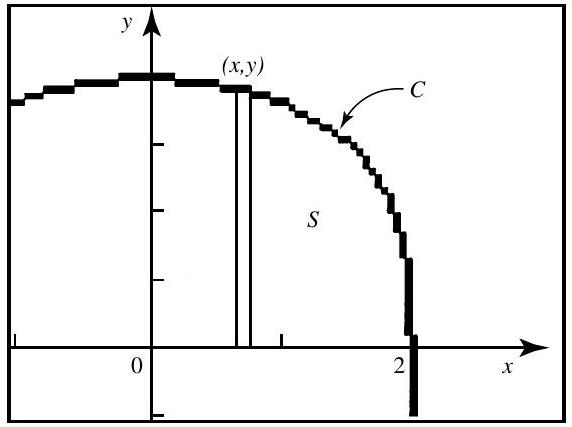
\includegraphics[width=0.40\linewidth]{calculus/images/71c445d1-6f5c-451e-be73-f2e2b89ae7db-08_427_572_1721_1078.jpg}
  \end{center}
  Graph $y=\sqrt[3]{\left(64-16 x^{2}\right)}$ in $[-1,3] \times[-1,5]$. Since you want $d y / d x$, the slope of the tangent, where $y=1$, use the calculator to solve
  \[
  \sqrt[3]{64-16 x^{2}}=1
  \]
  (storing the answer at B ). Then evaluate the slope of the tangent to $C$ at $y=1$ :
  \[
  f^{\prime}(B) \approx-21.182
  \]
\end{solutionorbox}

\item Find the area of $S$.
\begin{solutionorbox}[1in]
Since $\Delta A=y \Delta x, A=\int_{0}^{2} y d x \approx 6.730$.
\end{solutionorbox}

\item Find the volume generated when $S$ is rotated about the $x$-axis.
\begin{solutionorbox}[2in]
When $S$ is rotated about the $x$-axis, its volume can be obtained using disks:

\[
\begin{aligned}
\Delta V & =\pi R^{2} \Delta x=\pi y^{2} \Delta x \\
V & =\pi \int_{0}^{2} y^{2} d x \\
& =\pi \int_{0}^{2}\left(\sqrt[3]{64-16 x^{2}}\right)^{2} d x \approx 74.310
\end{aligned}
\]
\end{solutionorbox}
\end{enumerate}




\newpage




\question
Let $R$ be the point on the curve of $y=x-x^{2}$ such that the line $O R$ (where $O$ is the origin) divides the area bounded by the curve and the $x$-axis into two regions of equal area. Set up (but do not solve) an integral to find the $x$-coordinate of $R$.\\
\begin{solutionorbox}[2.5in]
See the figure, where $R$ is the point ( $a, b$ ), and seek $a$ such that
\[
\int_{0}^{a}\left(x-x^{2}-\dfrac{b}{a} \cdot x\right) d x=\dfrac{1}{2} \int_{0}^{1}\left(x-x^{2}\right) d x
\]
\begin{center}
  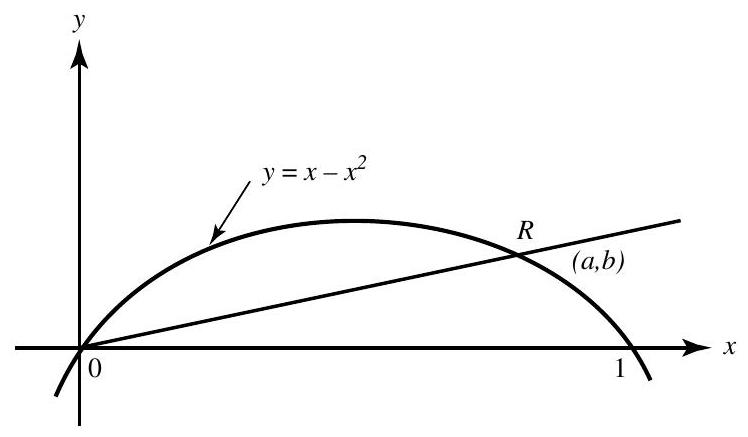
\includegraphics[width=0.40\linewidth]{calculus/images/71c445d1-6f5c-451e-be73-f2e2b89ae7db-09_437_748_932_614.jpg}
\end{center}
\end{solutionorbox}




\newpage



\question
Suppose $f^{\prime \prime}=\sin \left(2^{x}\right)$ for $-1<x<3.2$.
\begin{enumerate}
\renewcommand{\labelenumi}{(\alph{enumi})}
\item On what intervals is the graph of $f$ concave downward? Justify your answer.
\begin{solutionorbox}[1.5in]
  Graph $y=\sin 2^{x}$ in $[-1,3.2] \times[-1,1]$. Note that $y=f^{\prime \prime}$.\\
  \begin{center}
    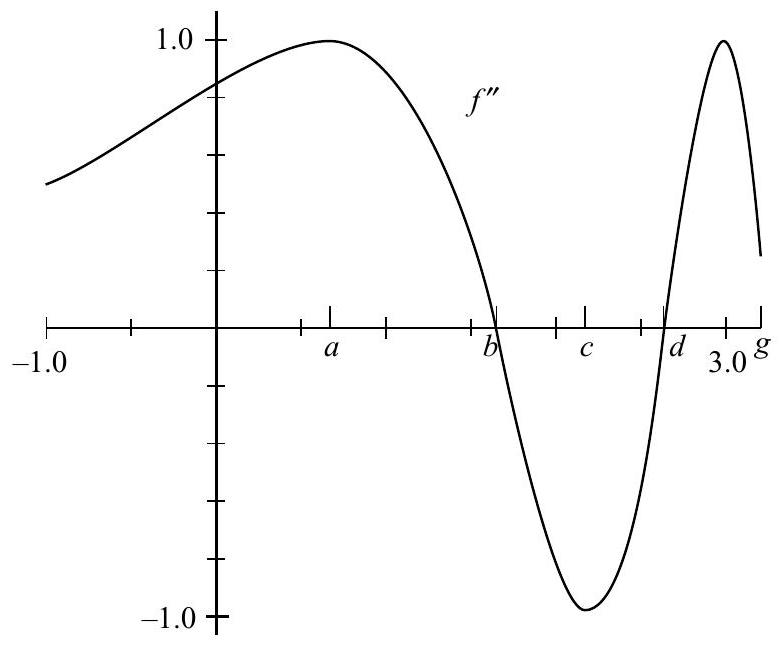
\includegraphics[width=0.40\linewidth]{calculus/images/71c445d1-6f5c-451e-be73-f2e2b89ae7db-09_648_783_1512_598.jpg}
  \end{center}
The graph of $f$ is concave downward where $f^{\prime \prime}$ is negative, namely, on ( $b, d$ ). Use the calculator to solve $\sin 2^{x}=0$, obtaining $b=1.651$ and $d=2.651$. The answer to (a) is therefore $1.651<x<2.651$.
\end{solutionorbox}
\item Find the $x$-coordinates of all relative minima of $f^{\prime}$.
\begin{solutionorbox}[1.5in]
$f^{\prime}$ has a relative minimum at $x=d$, because $f^{\prime \prime}$ equals 0 at $d$, is less than 0 on $(b, d)$, and is greater than 0 on $(d, g)$. Thus $f^{\prime}$ has a relative minimum (from part a) at 2.651.
\end{solutionorbox}
\item How many points of inflection does the graph of $f^{\prime}$ have? Justify your answer.
\begin{solutionorbox}[1.5in]
The graph of $f^{\prime}$ has a point of inflection wherever its second derivative $f^{\prime \prime \prime}$ changes from positive to negative or vice versa. This is equivalent to $f^{\prime \prime}$ changing from increasing to decreasing (as at $a$ and $g$ ) or vice versa (as at $c)$. Therefore, the graph of $f^{\prime}$ has three points of inflection on $[-1,3.2]$.
\end{solutionorbox}
\end{enumerate}





\newpage




\question
Let $f(x)=\cos x$ and $g(x)=x^{2}-1$.
\begin{enumerate}
\renewcommand{\labelenumi}{(\alph{enumi})}
\item Find the coordinates of any points of intersection of $f$ and $g$.
\begin{solutionorbox}[1in]
  Graph $f(x)=\cos x$ and $g(x)=x^{2}-1$ in $[-2,2] \times[-2,2]$. Here, $y_{1}=f$ and $y_{2}=g$.\\
  \begin{center}
    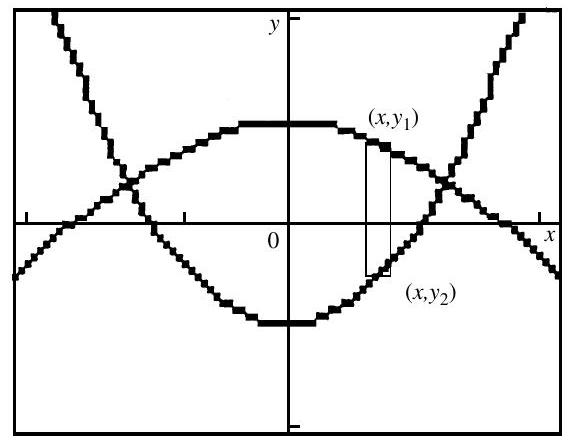
\includegraphics[width=0.40\linewidth]{calculus/images/71c445d1-6f5c-451e-be73-f2e2b89ae7db-10_444_570_380_1080.jpg}
  \end{center}
  Solve $\cos x=x^{2}-1$ to find the two points of intersection: $(1.177,0.384)$ and ( $-1.177,0.384$ ).
\end{solutionorbox}
\item Find the area bounded by $f$ and $g$.
\begin{solutionorbox}[2in]
Since $\Delta A=\left(y_{1}-y_{2}\right) \Delta x=[f(x)-g(x)] \Delta x$, the area $A$ bounded by the two curves is
\[
\begin{aligned}
A & =2 \int_{0}^{1.177}\left(y_{1}-y_{2}\right) d x \\
& =2 \int_{0}^{1.177}\left(\cos x-\left(x^{2}-1\right)\right) d x \\
& \approx 3.114
\end{aligned}
\]
\end{solutionorbox}
\end{enumerate}





\newpage





\question
\begin{enumerate}
\renewcommand{\labelenumi}{(\alph{enumi})}
\item In order to investigate mail-handling efficiency, each hour one morning a local post office checked the rate (letters/min) at which an employee was sorting mail. Use the results shown in the table to estimate the total number of letters he may have sorted that morning.

\begin{center}
\begin{tabular}{|l|c|c|c|c|c|}
\hline
Time & 8 & 9 & 10 & 11 & 12 \\
\hline
Letters/min & 10 & 12 & 8 & 9 & 11 \\
\hline
\end{tabular}
\end{center}
\begin{solutionorbox}[1.5in]
Use the Trapezoid Rule, with $h=60$ min:

\[
\begin{aligned}
& \dfrac{h}{2}\left(y_{0}+2 y_{1}+2 y_{2}+2 y_{3}+y_{4}\right)= \\
& \dfrac{60}{2}(10+2 \cdot 12+2 \cdot 8+2 \cdot 9+11)=2370 \text { letters. }
\end{aligned}
\]
\end{solutionorbox}

\item Hoping to speed things up a bit, the post office tested a sorting machine that can process mail at the constant rate of 20 letters per minute. The graph shows the rate at which letters arrived at the post office and were dumped into this sorter.
\begin{center}
  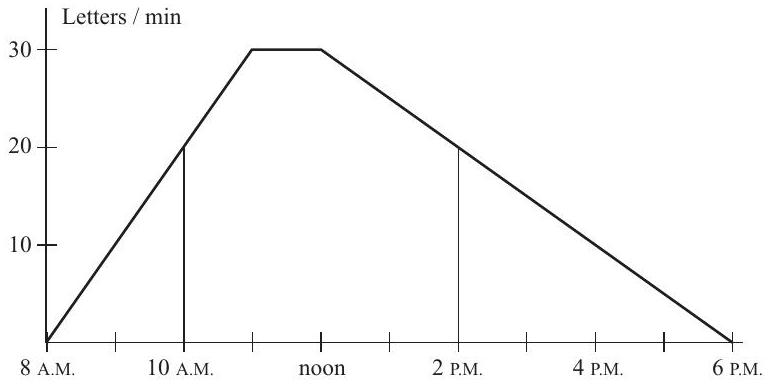
\includegraphics[width=0.40\linewidth]{calculus/images/71c445d1-6f5c-451e-be73-f2e2b89ae7db-02_389_773_2124_1004.jpg}
\end{center}
\begin{enumerate}
\renewcommand{\labelenumii}{(\roman{enumii})}
\item When did letters start to pile up?
\begin{solutionorbox}[2.5in]
Draw a horizontal line at $y=20$ (as shown on the graph below), representing the rate at which letters are processed then.
\begin{center}
  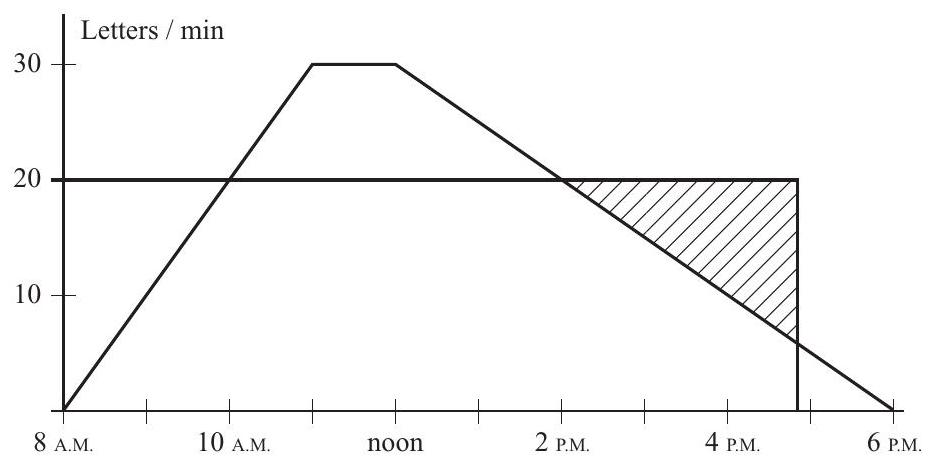
\includegraphics[width=0.40\linewidth]{calculus/images/71c445d1-6f5c-451e-be73-f2e2b89ae7db-10_467_933_1841_918.jpg}
\end{center}
Letters began to pile up when they arrived at a rate greater than that at which they were being processed, that is, at $t=10$ A.M.
\end{solutionorbox}

\item When was the pile the biggest?
\begin{solutionorbox}[1in]
The pile was largest when the letters stopped piling up, at $t=2$ p.m.
\end{solutionorbox}

\item How big was it then?
\begin{solutionorbox}[1in]
The number of letters in the pile is represented by the area of the small trapezoid above the horizontal line: $\dfrac{1}{2}(4 \cdot 60+1 \cdot 60)(10)=1500$.
\end{solutionorbox}

\item At about what time did the pile vanish?
\begin{solutionorbox}[1.5in]
The pile began to diminish after 2 P.M., when letters were processed at a rate faster than they arrived, and vanished when the area of the shaded triangle represented 1500 letters. At 5 p.m. this area is $\dfrac{1}{2}(3 \cdot 60)(10)=1800$ letters, so the pile vanished shortly before 5 P.M.
\end{solutionorbox}
\end{enumerate}
\end{enumerate}




\newpage




\question
A particle moves on the curve of $y^{3}=2 x+1$ so that its distance from the $x$-axis is increasing at the constant rate of 2 units $/ \mathrm{sec}$. When $t=0$, the particle is at $(0,1)$.
\begin{enumerate}
\renewcommand{\labelenumi}{(\alph{enumi})}
\item Find a pair of parametric equations $x=x(t)$ and $y=y(t)$ that describe the motion of the particle for nonnegative $t$.
\begin{solutionorbox}[1in]
Since $\dfrac{d y}{d t}=2, y=2 t+1$ and $x=4 t^{3}+6 t^{2}+3 t$.
\end{solutionorbox}
\item Find $|\mathbf{a}|$, the magnitude of the particle's acceleration, when $t=1$.
\begin{solutionorbox}[1in]
Since $\dfrac{d^{2} y}{d t^{2}}=0$ and $\dfrac{d^{2} x}{d t^{2}}=24 t+12$, then, when $t=1,|\mathbf{a}|=36$.
\end{solutionorbox}
\end{enumerate}



\question
Find the area of the region that the polar curves $r=2-\cos \theta$ and $r=3 \cos \theta$ enclose in common.\\
\begin{solutionorbox}[2.5in]
See the figure. The required area $A$ is twice the sum of the following areas: that of the limaon from 0 to $\dfrac{\pi}{3}$, and that of the circle from $\dfrac{\pi}{3}$ to $\dfrac{\pi}{2}$. Thus
\[
\begin{aligned}
A & =2\left[\dfrac{1}{2} \int_{0}^{\pi / 3}(2-\cos \theta)^{2} d \theta+\dfrac{1}{2} \int_{\pi / 3}^{\pi / 2}(3 \cos \theta)^{2} d \theta\right] \\
& =\dfrac{9 \pi}{4}-3 \sqrt{3}
\end{aligned}
\]
\begin{center}
  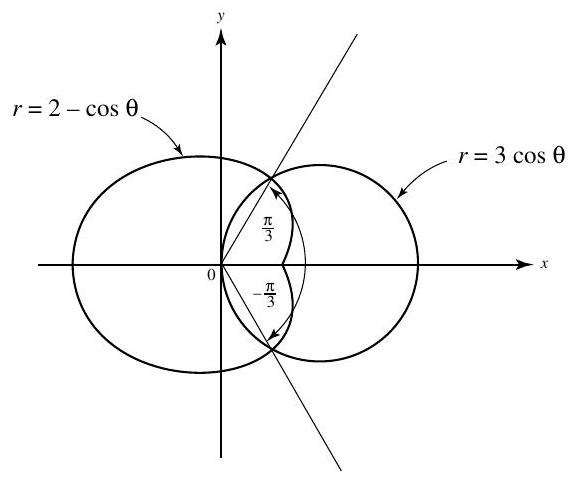
\includegraphics[width=0.40\linewidth]{calculus/images/71c445d1-6f5c-451e-be73-f2e2b89ae7db-11_482_576_1233_730.jpg}
\end{center}
\end{solutionorbox}





\newpage




\question
\begin{enumerate}
\renewcommand{\labelenumi}{(\alph{enumi})}
\item Using your calculator, verify that
\[
\left(4 \tan ^{-1}(1 / 5)\right)-\left(\tan ^{-1}(1 / 239)\right) \approx \dfrac{\pi}{4} .
\]
\begin{solutionorbox}[1in]
Both $\pi / 4$ and the expression in brackets yield 0.7853981634 , which is accurate to ten decimal places.
\end{solutionorbox}
\item Use the Taylor polynomial of degree 7 about 0 ,
\[
\tan ^{-1} x \approx x-x^{3} / 3+x^{5} / 5-x^{7} / 7,
\]
to approximate $\tan ^{-1} 1 / 5$, and the polynomial of degree 1 to approximate $\tan ^{-1} 1 / 239$.
\begin{solutionorbox}[1.5in]
$\tan ^{-1} \dfrac{1}{5}=\dfrac{1}{5}-\dfrac{1}{3}\left(\dfrac{1}{5}\right)^{3}+\dfrac{1}{5}\left(\dfrac{1}{5}\right)^{5}-\dfrac{1}{7}\left(\dfrac{1}{5}\right)^{7}=0.197396$.
\[
\tan ^{-1} \dfrac{1}{239}=\dfrac{1}{239}=0.004184
\]
\end{solutionorbox}
\item Use part (b) to evaluate the expression in (a).
\begin{solutionorbox}[1.5in]
$4 \tan ^{-1} \dfrac{1}{5}-\tan ^{-1} \dfrac{1}{239}=0.7854$; this agrees with the value of $\dfrac{\pi}{4}$ to four decimal places.
\end{solutionorbox}

\item Explain how the approximation for $\pi / 4$ given here compares with that obtained using $\pi / 4=\tan ^{-1} 1$.
\begin{solutionorbox}[1.5in]
The series
\[
\tan ^{-1} 1=1-\dfrac{1}{3}+\dfrac{1}{5}-\dfrac{1}{7}+\cdots
\]
converges very slowly. Example 56, page 436, evaluated the sum of 60 terms of the series for $\pi$ (which equals $4 \tan ^{-1} 1$ ). To four decimal places, we get $\pi=3.1249$, which yields 0.7812 for $\pi / 4$ not accurate even to two decimal places.
\end{solutionorbox}
\end{enumerate}





\newpage





\question
\begin{enumerate}
\renewcommand{\labelenumi}{(\alph{enumi})}
\item Show that the series $\sum_{n=1}^{\infty}(-1)^{n+1} \dfrac{1}{\ln (n+1)}$ converges.
\begin{solutionorbox}[1.5in]
The given series is alternating. Since $\lim\limits_{n \to \infty} \ln (n+1)=\infty, \lim\limits_{n \to \infty} \dfrac{1}{\ln (n+1)}=0$.

Since $\ln x$ is an increasing function,

\[
\ln (n+1)>\ln n \quad \text { and } \quad \dfrac{1}{\ln (n+1)}<\dfrac{1}{\ln n}
\]

The series therefore converges.
\end{solutionorbox}

\item How many terms of the series are needed to get a partial sum within 0.1 of the sum of the whole series?
\begin{solutionorbox}[2in]
Since the series converges by the Alternating Series Test, the error in using the first $n$ terms for the sum of the whole series is less than the absolute value of the $(n+1)$ st term. Thus the error is less than $\dfrac{1}{\ln (n+1)}$. Solve for $n$ using $\dfrac{1}{\ln (n+1)}<0.1$ :

\[
\begin{aligned}
\ln (n+1) & >10 \\
(n+1) & >e^{10} \\
n & >e^{10}-1>22,025
\end{aligned}
\]

The given series converges very slowly!
\end{solutionorbox}

\item Tell whether the series $\sum_{n=2}^{\infty}(-1)^{n} \dfrac{1}{n \ln n}$ is absolutely convergent, conditionally convergent, or divergent. Justify your answer.
\begin{solutionorbox}[1.5in]
The series $\sum_{2}^{\infty}(-1)^{n} \dfrac{1}{n \ln n}$ is conditionally convergent. The given alternating series converges since the $n$th term approaches 0 and $\dfrac{1}{(n+1) \ln (n+1)}<\dfrac{1}{n \ln n}$. However, the nonnegative series diverges by the Integral Test, since
\[
\int_{2}^{\infty} \dfrac{1}{x \ln x} d x=\left.\lim\limits_{b \to \infty} \ln (\ln x)\right|_{2} ^{b}=\infty
\]
\end{solutionorbox}
\end{enumerate}





\newpage





\question
Given $\dfrac{d y}{d t}=k y(10-y)$ with $y=2$ at $t=0$ and $y=5$ at $t=2$ :
\begin{enumerate}
\renewcommand{\labelenumi}{(\alph{enumi})}
\item Find $k$.
\begin{solutionorbox}[2in]
Solve by separation of variables:
\[
\begin{gathered}
\dfrac{d y}{y(10-y)}=k d t \\
\dfrac{1}{10} \int\left(\dfrac{1}{y}+\dfrac{1}{10-y}\right) d y=\int k d t \\
\dfrac{1}{10} \ln \left(\dfrac{y}{10-y}\right)=k t+C \\
\ln \left(\dfrac{10-y}{y}\right)=-10(k t+C)
\end{gathered}
\]
Let $c=e^{-10 C}$; then
\[
\dfrac{10-y}{y}=c e^{-10 k t}
\]
Now use initial condition $y=2$ at $t=0$ :
\[
\dfrac{8}{2}=c e^{0} \text { so } c=4
\]
and the other condition, $y=5$ at $t=2$, gives
\[
\dfrac{5}{5}=4 e^{-20 k} \text { or } k=\dfrac{1}{10} \ln 2 .
\]
\end{solutionorbox}
\item Express $y$ as a function of $t$.
\begin{solutionorbox}[1.5in]
Since $c=4$ and $k=\dfrac{1}{10} \ln 2$, then $\dfrac{10-y}{y}=4 e^{-10\left(\dfrac{1}{10} \ln 2\right) t}$. Solving for $y$ yields
\[
y=\dfrac{10}{1+4 \cdot 2^{-t}}
\]
\end{solutionorbox}
\item For what value of $t$ will $y=8$ ?
\begin{solutionorbox}[1in]
$8=\dfrac{10}{1+4 \cdot 2^{-t}}$ means $1+4 \cdot 2^{-t}=1.25$, so $t=4$.
\end{solutionorbox}
\item Describe the long-range behavior of $y$.
\begin{solutionorbox}[1in]
$\lim\limits_{t \to \infty} \dfrac{10}{1+4 \cdot 2^{-t}}=10$, so the value of $y$ approaches 10 .
\end{solutionorbox}
\end{enumerate}






\newpage






\question
An object $P$ is in motion in the first quadrant along the parabola $y=18-2 x^{2}$ in such a way that at $t \sec$ the abscissa of its position is $x=\dfrac{1}{2} t$.

\begin{enumerate}
\renewcommand{\labelenumi}{(\alph{enumi})}
\item Where is $P$ when $t=4$ ?
\begin{solutionorbox}[1in]
Since $x=\dfrac{1}{2} t, x(4)=\dfrac{1}{2}(4)=2$. Since $y=18-2 \cdot 2^{2}=10, P$ is at $(2,10)$.
\end{solutionorbox}

\item What is the vertical component of its velocity there?
\begin{solutionorbox}[1.5in]
Since $y=18-2 x^{2}, \dfrac{d y}{d t}=-4 x \dfrac{d x}{d t}$. Since $x=\dfrac{1}{2} t, \dfrac{d x}{d t}=\dfrac{1}{2}$. Therefore $\dfrac{d y}{d t}=-4 x \dfrac{d x}{d t}=-4 \cdot 2 \cdot \dfrac{1}{2}=-4$ unit $/ \mathrm{sec}$.
\end{solutionorbox}

\item At what rate is its distance from the origin changing then?
\begin{solutionorbox}[2in]
Let $D=$ the object's distance from the origin. Then

\[
\begin{aligned}
D^{2}=x^{2}+y^{2} & , \text { and at }(2,10) D=\sqrt{104} \\
2 D \dfrac{d D}{d t} & =2 x \dfrac{d x}{d t}+2 y \dfrac{d y}{d t} \\
2 \sqrt{104} \dfrac{d D}{d t} & =2 \cdot 2 \cdot \dfrac{1}{2}+2 \cdot 10(-4) \\
\dfrac{d D}{d t} & =\dfrac{-78}{2 \sqrt{104}}=-3.824 \mathrm{unit} / \mathrm{sec}
\end{aligned}
\]
\end{solutionorbox}

\item When does it hit the $x$-axis?
\begin{solutionorbox}[1.5in]
The object hits the $x$-axis when $y=18-2 x^{2}=0$, or $x=3$. Since

\[
x=\dfrac{1}{2} t=3, t=6
\]
\end{solutionorbox}

\item How far did it travel altogether?
\begin{solutionorbox}[1.5in]
The length of the arc of $y=18-2 x^{2}$ for $0 \leq x \leq 3$ is given by

\[
L=\int \sqrt{1+\left(\dfrac{d y}{d x}\right)^{2}} d x=\int_{0}^{3} \sqrt{1+(-4 x)^{2}} d x=18.460 \text { units. }
\]
\end{solutionorbox}
\end{enumerate}






\newpage




\question
A particle moves in the $x y$-plane in such a way that at any time $t \geq 0$ its position is given by $x(t)=4 \arctan t, y(t)=\dfrac{12 t}{t^{2}+1}$.

\begin{enumerate}
\renewcommand{\labelenumi}{(\alph{enumi})}
\item Sketch the path of the particle, indicating the direction of motion.
\begin{solutionorbox}[2.5in]
See graph.
\begin{center}
  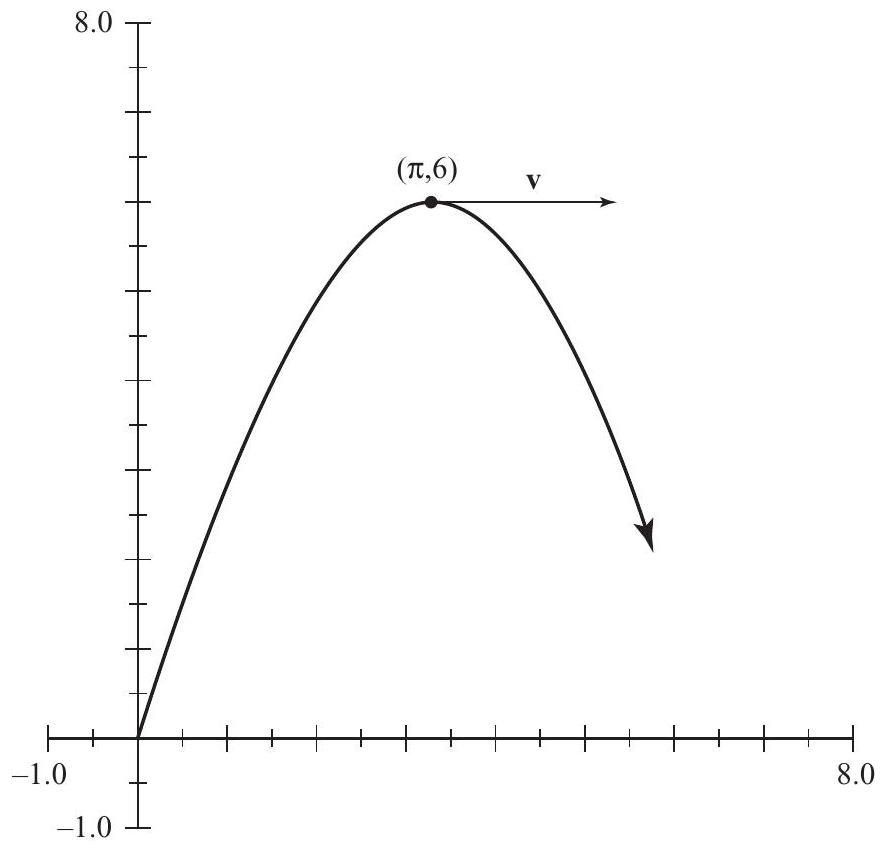
\includegraphics[width=0.40\linewidth]{calculus/images/71c445d1-6f5c-451e-be73-f2e2b89ae7db-14_848_887_375_941.jpg}
\end{center}
\end{solutionorbox}

\item At what time $t$ does the particle reach its highest point? Justify.
\begin{solutionorbox}[2.5in]
You want to maximize $y(t)=\dfrac{12 t}{t^{2}+1}$.


\[
y^{\prime}(t)=\dfrac{\left(t^{2}+1\right)(12)-12 t(2 t)}{\left(t^{2}+1\right)^{2}}=\dfrac{12(1-t)(1+t)}{\left(t^{2}+1\right)^{2}} .
\]

See signs analysis.\\
\begin{center}
  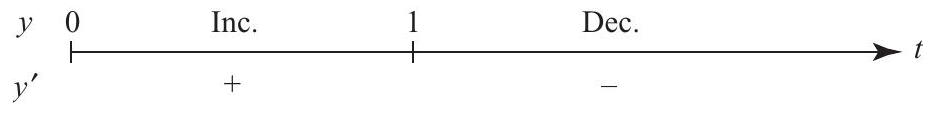
\includegraphics[width=0.40\linewidth]{calculus/images/71c445d1-6f5c-451e-be73-f2e2b89ae7db-14_113_934_1609_957.jpg}
\end{center}

The maximum $y$ occurs when $t=1$, because $y$ changes from increasing to decreasing there.\\
\end{solutionorbox}

\item Find the coordinates of that highest point, and sketch the velocity vector there.
\begin{solutionorbox}[1.5in]
Since $x(1)=4 \arctan 1=\pi$ and $y(1)=\dfrac{12}{1+1}=6$, the coordinates of the highest point are $(\pi, 6)$.

Since $x^{\prime}(t)=\dfrac{4}{1+t^{2}}$ and $y^{\prime}(t)=\dfrac{12\left(1-t^{2}\right)}{\left(t^{2}+1\right)^{2}}$, so $\mathbf{v}(1)=(2,0)$. This vector is shown on the graph.
\end{solutionorbox}

\item Describe the long-term behavior of the particle.
\begin{solutionorbox}[1.5in]
$\lim\limits_{t \to \infty} x(t)=\lim\limits_{t \to \infty} 4 \arctan t=4\left(\dfrac{\pi}{2}\right)=2 \pi$, and $\lim\limits_{t \to \infty} y(t)=\lim\limits_{t \to \infty} \dfrac{12 t}{t^{2}+1}=0$. Thus the particle approaches the point $(2 \pi, 0)$.
\end{solutionorbox}
\end{enumerate}





\newpage





\question
The figure below shows the graph of $f^{\prime}$, the derivative of $f$, with domain $-3 \leq x \leq 9$. The graph of $f^{\prime}$ has horizontal tangents at $x=2$ and $x=4$, and a corner at $x=6$.\\
\begin{center}
  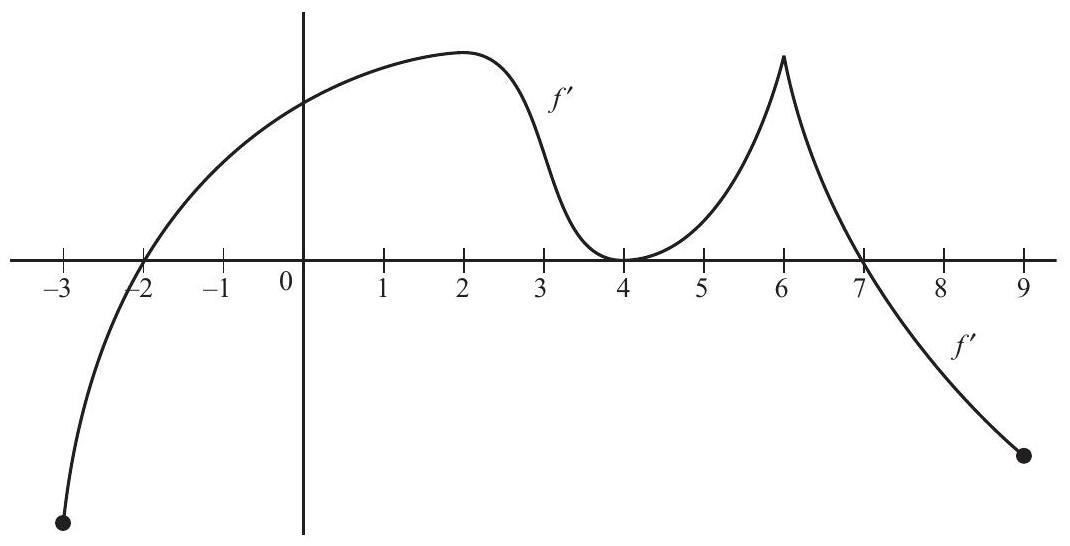
\includegraphics[width=0.70\linewidth]{calculus/images/71c445d1-6f5c-451e-be73-f2e2b89ae7db-04_546_1070_524_858.jpg}
\end{center}
\begin{enumerate}
\renewcommand{\labelenumi}{(\alph{enumi})}
\item Is $f$ continuous? Explain.
\begin{solutionorbox}[1in]
$f^{\prime}$ is defined for all $x$ in the interval. Since $f$ is therefore differentiable, it must also be continuous.
\end{solutionorbox}
\item Find all values of $x$ at which $f$ attains a relative minimum. Justify.
\begin{solutionorbox}[1.5in]
From the graph we see that $f^{\prime}=0$ at $x=-2,4$, and 7. The sign of $f^{\prime}$ tells whether $f$ is increasing or decreasing on the relevant intervals. $f$ attains relative minima at $x=-2$ and $x=9$.
\end{solutionorbox}
\item Find all values of $x$ at which $f$ attains a relative maximum. Justify.
\begin{solutionorbox}[1in]
Similarly, $f$ attains relative maxima at $x=-3$ and $x=7$.
\end{solutionorbox}
\item At what value of $x$ does $f$ attain its absolute maximum? Justify.
\begin{solutionorbox}[1.5in]
Note that $f(7)-f(-3)=\int_{-3}^{7} f^{\prime}(x) d x$. Since there is more area above the $x$-axis than below the $x$-axis on $[-3,7]$, the integral is positive and $f(7)-f(-3)>0$. This implies that $f(7)>f(-3)$, and that the absolute maximum occurs at $x=7$.
\end{solutionorbox}
\item Find all values of $x$ at which the graph of $f$ has a point of inflection. Justify.
\begin{solutionorbox}[1.5in]
Since $f^{\prime}$ changes from increasing to decreasing (or vice versa) at $x=2,4$, and $6, f^{\prime \prime}$ changes sign at each of these points. Therefore, the graph of $f$ has points of inflection there.
\end{solutionorbox}
\end{enumerate}





\newpage





\question
Find the area of the largest rectangle (with sides parallel to the coordinate axes) that can be inscribed in the region bounded by the graphs of $f(x)=8-2 x^{2}$ and $g(x)=x^{2}-4$.\\
\begin{solutionorbox}[1.5in]
Draw a sketch of the region bounded above by $y_{1}=8-2 x^{2}$ and below by $y_{2}=x^{2}-4$, and inscribe a rectangle in this region as described in the question. If $\left(x, y_{1}\right)$ and $\left(x, y_{2}\right)$ are the vertices of the rectangle in quadrants I and IV, respectively, then the area
\[
A=2 x\left(y_{1}-y_{2}\right)=2 x\left(12-3 x^{2}\right), \text { or } A(x)=24 x-6 x^{3}
\]
Then $A^{\prime}(x)=24-18 x^{2}=6\left(4-3 x^{2}\right)$, which equals 0 when $x=\dfrac{2}{\sqrt{3}}=\dfrac{2 \sqrt{3}}{3}$.\\
Check to verify that $A^{\prime \prime}(x)<0$ at this point. This assures that this value of $x$ yields maximum area, which is given by $\dfrac{4 \sqrt{3}}{3} \times 8$.
\end{solutionorbox}





\newpage




\question
Given the graph of $f(x)$, sketch the graph of $f^{\prime}(x)$.\\
\begin{center}
  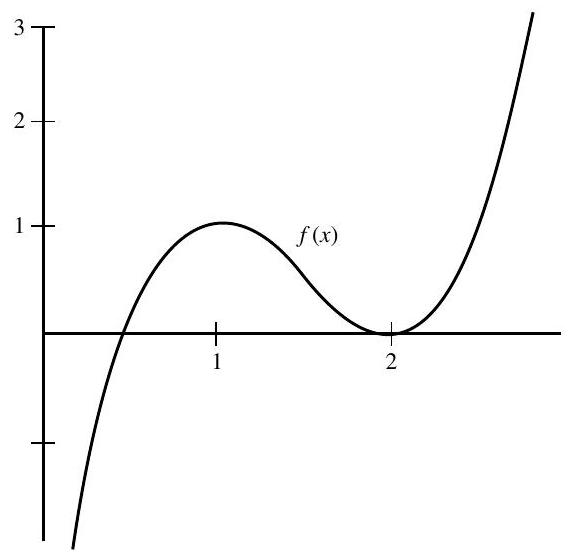
\includegraphics[width=0.40\linewidth]{calculus/images/71c445d1-6f5c-451e-be73-f2e2b89ae7db-04_558_574_1625_1099.jpg}
\end{center}
\begin{solutionorbox}[2.5in]
The graph of $f^{\prime}(x)$ is shown here.\\
\begin{center}
  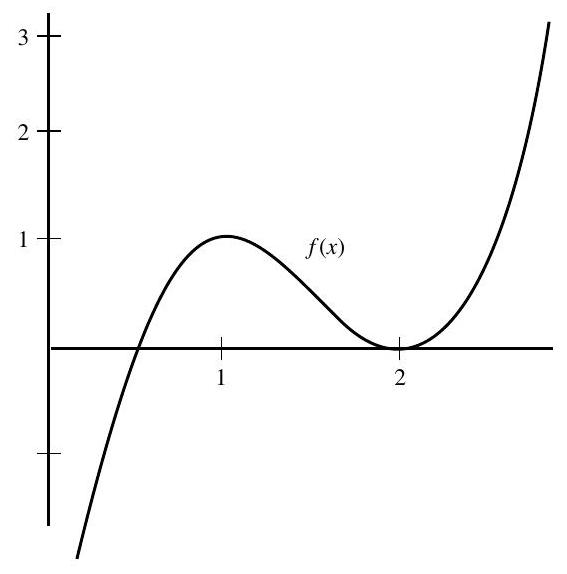
\includegraphics[width=0.40\linewidth]{calculus/images/71c445d1-6f5c-451e-be73-f2e2b89ae7db-15_574_567_1730_433.jpg}
\end{center}
\begin{center}
  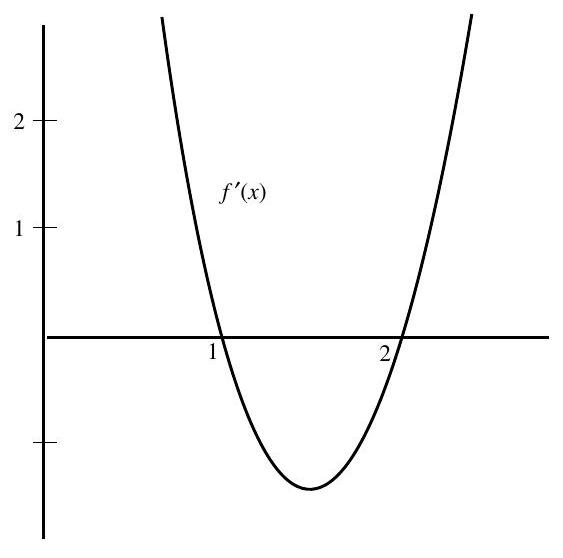
\includegraphics[width=0.40\linewidth]{calculus/images/71c445d1-6f5c-451e-be73-f2e2b89ae7db-15_558_563_1739_1080.jpg}
\end{center}
\end{solutionorbox}




\newpage





\question
A cube is contracting so that its surface area decreases at the constant rate of $72 \mathrm{in} .^{2} / \mathrm{sec}$. Determine how fast the volume is changing at the instant when the surface area is $54 \mathrm{ft}^{2}$.\\
\begin{solutionorbox}[1.5in]
The rate of change in volume when the surface area is $54 \mathrm{ft}^{2}$ is $-\dfrac{3}{8} \mathrm{ft}^{3} / \mathrm{sec}$.
\end{solutionorbox}


\question
A square is inscribed in a circle of radius $a$ as shown in the diagram. Find the volume obtained if the region outside the square but inside the circle is rotated about a diagonal of the square.\\
\begin{center}
  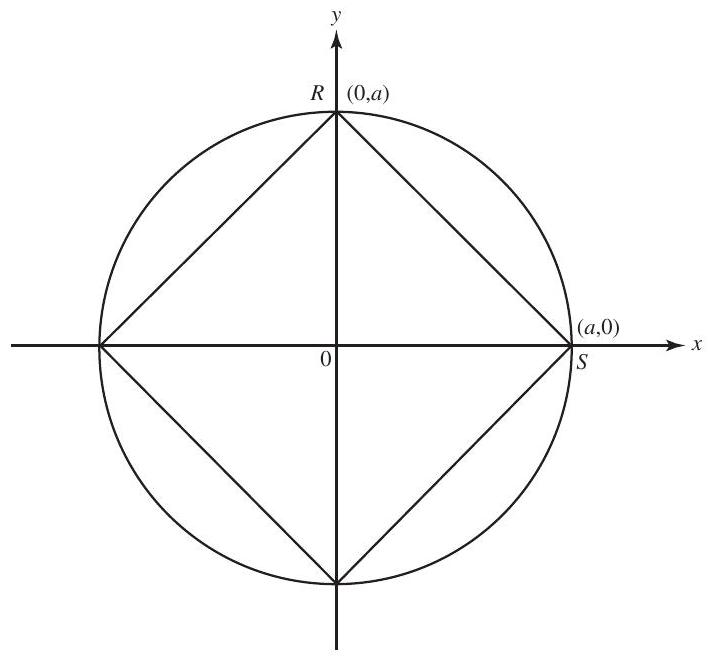
\includegraphics[width=0.40\linewidth]{calculus/images/71c445d1-6f5c-451e-be73-f2e2b89ae7db-05_657_711_473_677.jpg}
\end{center}
\begin{solutionorbox}[2.5in]
See the figure. The equation of the circle is $x^{2}+y^{2}=a^{2}$; the equation of $R S$ is $y=a-x$. If $y_{2}$ is an ordinate of the circle and $y_{1}$ of the line, then,
\[
\begin{gathered}
\Delta V=\pi y_{2}^{2} \Delta x-\pi y_{1}^{2} \Delta x \\
V=2 \pi \int_{0}^{a}\left[\left(a^{2}-x^{2}\right)-(a-x)^{2}\right] d x=\dfrac{2}{3} \pi a^{3}
\end{gathered}
\]
\begin{center}
  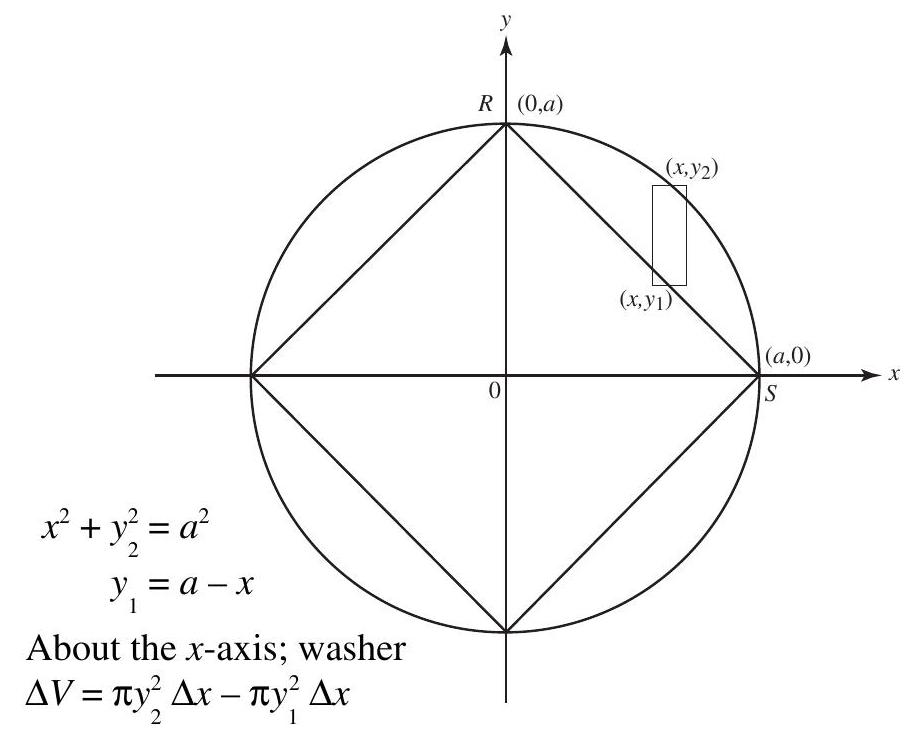
\includegraphics[width=0.40\linewidth]{calculus/images/71c445d1-6f5c-451e-be73-f2e2b89ae7db-16_736_920_707_867.jpg}
\end{center}
\end{solutionorbox}





\newpage




\question
\begin{enumerate}
\renewcommand{\labelenumi}{(\alph{enumi})}
\item Sketch the region in the first quadrant bounded above by the line $y=x+4$, below by the line $y=4-x$, and to the right by the parabola $y=x^{2}+2$.
\begin{solutionorbox}[2.5in]
The region is sketched in the figure. The pertinent points of intersection are labeled.
\begin{center}
  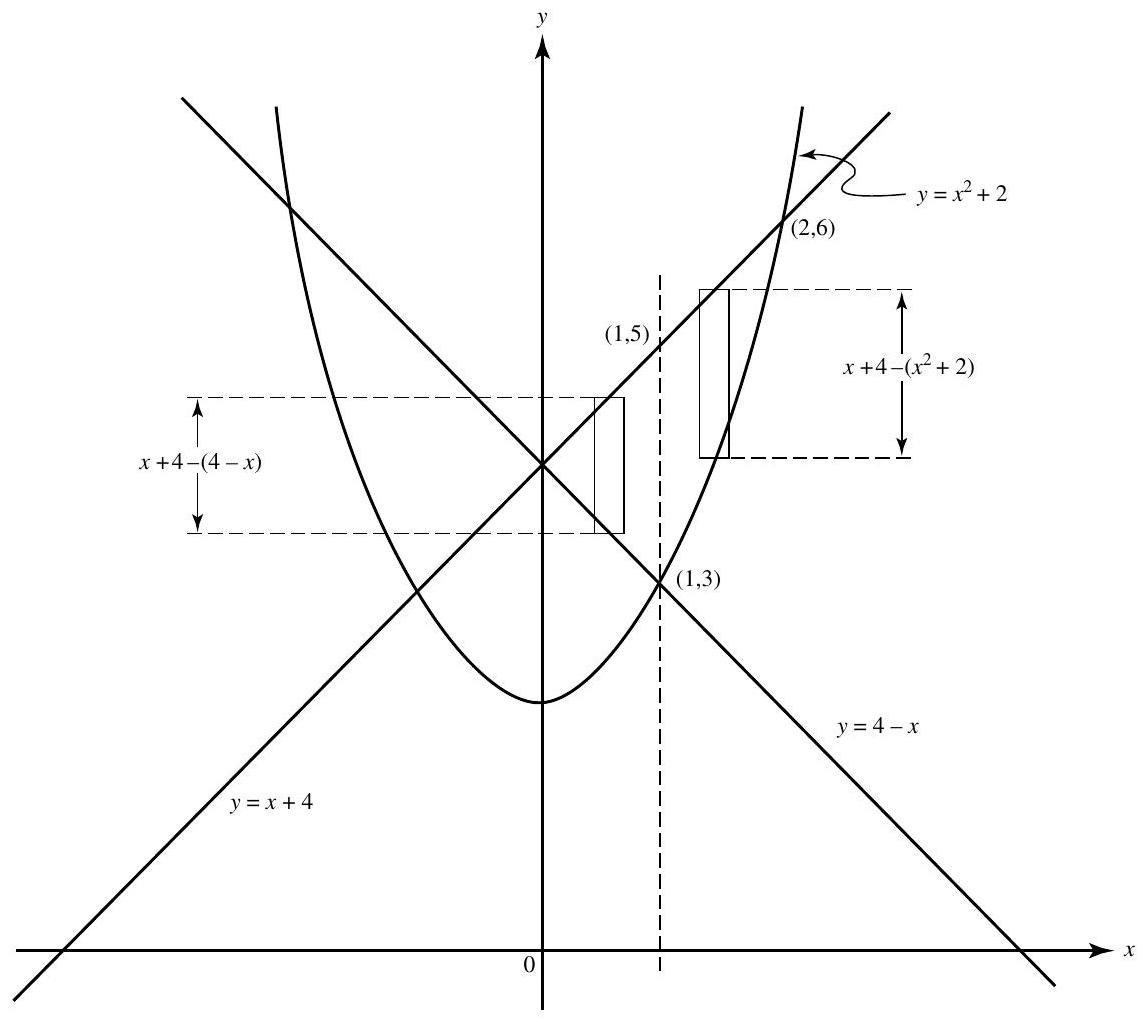
\includegraphics[width=0.40\linewidth]{calculus/images/71c445d1-6f5c-451e-be73-f2e2b89ae7db-16_1022_1147_1639_807.jpg}
\end{center}
\end{solutionorbox}
\item Find the area of this region.
\begin{solutionorbox}[1.5in]
The required area consists of two parts. The area of the triangle is represented by $\int_{1}^{2}[(x+4)-(4-x)] d x$ and is equal to 1 , while the area of the region bounded at the left by $x=1$, above by $y=x+4$, and at the right by the parabola is represented by $\int_{1}^{2}\left[(x+4)-\left(x^{2}+2\right)\right] d x$. This equals
\[
\int_{1}^{2}\left(x+2-x^{2}\right) d x=\dfrac{x^{2}}{2}+2 x-\left.\dfrac{x^{3}}{3}\right|_{1} ^{2}=\dfrac{7}{6}
\]
The required area, thus, equals $2 \dfrac{1}{6}$ or $\dfrac{13}{6}$.
\end{solutionorbox}
\end{enumerate}





\newpage





\question
The graph shown below is based roughly on data from the U.S. Department of Agriculture.\\
\begin{center}
  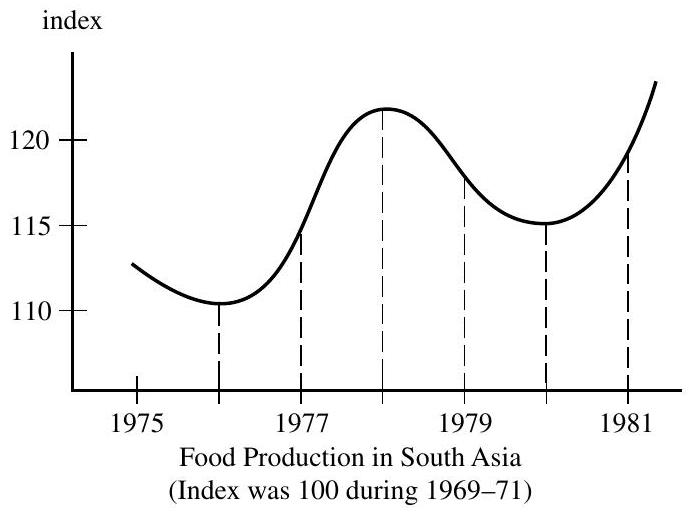
\includegraphics[width=0.40\linewidth]{calculus/images/71c445d1-6f5c-451e-be73-f2e2b89ae7db-05_514_692_1484_679.jpg}
\end{center}
\begin{enumerate}
\renewcommand{\labelenumi}{(\alph{enumi})}
\item During which intervals did food production decrease in South Asia?
\begin{solutionorbox}[1in]
1975 to 1976 and 1978 to 1980.
\end{solutionorbox}

\item During which intervals did the rate of change of food production increase?
\begin{solutionorbox}[1in]
1975 to 1977 and 1979 to 1981.
\end{solutionorbox}

\item During which intervals did the increase in food production accelerate?
\begin{solutionorbox}[1in]
1976 to 1977 and 1980 to 1981.
\end{solutionorbox}
\end{enumerate}






\newpage




\question
A particle moves along a straight line so that its acceleration at any time $t$ is given in terms of its velocity $v$ by $a=-2 v$.

\begin{enumerate}
\renewcommand{\labelenumi}{(\alph{enumi})}
\item Find $v$ in terms of $t$ if $v=20$ when $t=0$.
\begin{solutionorbox}[2in]
Since $a=\dfrac{d v}{d t}=-2 v$, then, separating variables, $\dfrac{d v}{v}=-2 d t$. Integrating gives
\begin{equation*}
\ln v=-2 t+C \tag{1}
\end{equation*}
and, since $v=20$ when $t=0, C=\ln 20$. Then (1) becomes $\ln \dfrac{v}{20}=-2 t$ or, solving for $v$,
\begin{equation*}
v=20 e^{-2 t} \tag{2}
\end{equation*}
\end{solutionorbox}
\item Find the distance the particle travels while $v$ changes from $v=20$ to $v=5$.
\begin{solutionorbox}[2in]
Note that $v>0$ for all $t$. Let $s$ be the required distance traveled (as $v$ decreases from 20 to 5); then
\begin{equation*}
s=\int_{v=20}^{v=5} 20 e^{-2 t} d t=\int_{t=20}^{\ln 2} 20 e^{-2 t} d t \tag{3}
\end{equation*}
where, when $v=20, t=0$. Also, when $v=5$, use (2) to get $\dfrac{1}{4}=e^{-2 t}$ or $-\ln 4=-2 t$. So $t=\ln 2$. Evaluating $s$ in (3) gives
\[
s=-\left.10 e^{-2 t}\right|_{0} ^{\ln 2}=-10\left(\dfrac{1}{4}-1\right)=\dfrac{15}{2} .
\]
\end{solutionorbox}
\end{enumerate}



\question
Let $R$ represent the region bounded above by the parabola $y=27-x^{2}$ and below by the $x$-axis. Isosceles triangle $A O B$ is inscribed in region $R$ with its vertex at the origin $O$ and its base $\overline{A B}$ parallel to the $x$-axis. Find the maximum possible area for such a triangle.\\
\begin{solutionorbox}[1.5in]
Let $(x, y)$ be the point in the first quadrant where the line parallel to the $x$-axis meets the parabola. The area of the triangle is given by
\[
A=x y=x\left(27-x^{2}\right)=27 x-x^{3} \text { for } 0 \leq x \leq 3 \sqrt{3} .
\]
Then $A^{\prime}(x)=27-3 x^{2}=3(3+x)(3-x)$, and $A^{\prime}(x)=0$ at $x=3$.\\
Since $A^{\prime}$ changes from positive to negative at $x=3$, the area reaches its maximum there.\\
The maximum area is $A(3)=3\left(27-3^{2}\right)=54$.
\end{solutionorbox}





\newpage




\question
\begin{enumerate}
\renewcommand{\labelenumi}{(\alph{enumi})}
\item Find the Maclaurin series for $f(x)=\ln (1+x)$.
\begin{solutionorbox}[2in]
Let $f(x)=\ln (1+x)$. Then $f^{\prime}(x)=\dfrac{1}{1+x}, f^{\prime \prime}(x)=-\dfrac{1}{(1+x)^{2}}, f^{\prime \prime \prime}(x)=\dfrac{2}{(1+x)^{3}}$,
\[
\begin{gathered}
f^{(4)}(x)=-\dfrac{3!}{(1+x)^{4}}, f^{(5)}(x)=\dfrac{4!}{(1+x)^{5}} \text {. At } x=0, \\
f(0)=0, f^{\prime}(0)=1, f^{\prime \prime}(0)=-1, f^{\prime \prime \prime}(0)=2, f^{(4)}(0)=-(3!), \text { and } f^{(5)}(0)=4!. \text { So } \\
\ln (1+x)=x-\dfrac{x^{2}}{2}+\dfrac{x^{3}}{3}-\dfrac{x^{4}}{4}+\dfrac{x^{5}}{5}-\cdots
\end{gathered}
\]
\end{solutionorbox}
\item What is the radius of convergence of the series in (a)?
\begin{solutionorbox}[1.5in]
Using the Ratio Test, you know that the series converges when $\lim\limits_{x \to \infty}\left|\dfrac{x^{n+1}}{n+1} \cdot \dfrac{n}{x^{n}}\right|<1$, that is, when $|x|<1$, or $-1<x<1$. Thus, the radius of convergence is 1 .
\end{solutionorbox}
\item Use the first five terms in (a) to approximate $\ln (1.2)$.
\begin{solutionorbox}[1in]
$\ln (1.2)=0.2-\dfrac{(0.2)^{2}}{2}+\dfrac{(0.2)^{3}}{3}+\dfrac{(0.2)^{4}}{4}+\dfrac{(0.2)^{5}}{5}$.
\end{solutionorbox}
\item Estimate the error in (c), justifying your answer.
\begin{solutionorbox}[1.5in]
Since the series converges by the Alternating Series Test, the error in the answer for (c) is less absolutely than $\dfrac{(0.2)^{6}}{6}$.
\end{solutionorbox}
\end{enumerate}



\question
A cycloid is given parametrically by $x=\theta-\sin \theta, y=1-\cos \theta$.
\begin{enumerate}
\renewcommand{\labelenumi}{(\alph{enumi})}
\item Find the slope of the curve at the point where $\theta=\dfrac{2 \pi}{3}$.
\begin{solutionorbox}[1.5in]
From the equations for $x$ and $y$,
\[
d x=(1-\cos \theta) d \theta \quad \text { and } \quad d y=\sin \theta d \theta
\]
The slope at any point is given by $\dfrac{d y}{d x}$, which here is $\dfrac{\sin \theta}{1-\cos \theta}$. When $\theta=\dfrac{2 \pi}{3}$, the slope is $\dfrac{\sqrt{3}}{3}$.
\end{solutionorbox}
\item Find the equation of the tangent to the cycloid at the point where $\theta=\dfrac{2 \pi}{3}$.
\begin{solutionorbox}[1.5in]
When $\theta=\dfrac{2 \pi}{3}, x=\dfrac{2 \pi}{3}-\dfrac{\sqrt{3}}{2}$ and $y=1-\left(-\dfrac{1}{2}\right)=\dfrac{3}{2}$. The equation of the tangent is $9 y-3 \sqrt{3} \cdot x=18-2 \pi \sqrt{3}$.
\end{solutionorbox}
\end{enumerate}






\newpage




\question
Find the area of the region enclosed by both the polar curves $r=4 \sin \theta$ and $r=4 \cos \theta$.\\
\begin{solutionorbox}[1.5in]
Both curves are circles with centers at, respectively, $(2,0)$ and $\left(2, \dfrac{\pi}{2}\right)$; the circles intersect at $\left(2 \sqrt{2}, \dfrac{\pi}{4}\right)$. The common area is given by

\[
\int_{0}^{\pi / 4}(4 \sin \theta)^{2} d \theta \text { or } \int_{\pi / 4}^{\pi / 2}(4 \cos \theta)^{2} d \theta
\]

The answer is $2(\pi-2)$.
\end{solutionorbox}


\question
\begin{enumerate}
\renewcommand{\labelenumi}{(\alph{enumi})}
\item Find the 4th degree Taylor polynomial about 0 for $\cos x$.
\begin{solutionorbox}[1.5in]
For $f(x)=\cos x, f^{\prime}(x)=-\sin x, f^{\prime \prime}(x)=-\cos x, f^{\prime \prime \prime}(x)=\sin x, f^{(4)}(x)=\cos x$, $f^{(5)}(x)=-\sin x, f^{(6)}(x)=-\cos x$. The Taylor polynomial of order 4 about 0 is

\[
\cos x=1-\dfrac{x^{2}}{2!}+\dfrac{x^{4}}{4!}
\]

Note that the next term of the alternating Maclaurin series for $\cos x$ is $-\dfrac{x^{6}}{6!}$.
\end{solutionorbox}

\item Use part (a) to evaluate $\int_{0}^{1} \cos x d x$.
\begin{solutionorbox}[1.5in]
$\int_{0}^{1} \cos x d x=x-\dfrac{x^{3}}{3 \cdot 2!}+\left.\dfrac{x^{5}}{5 \cdot 4!}\right|_{0} ^{1}=1-\dfrac{1}{6}+\dfrac{1}{120}$.
\end{solutionorbox}

\item Estimate the error in (b), justifying your answer.
\begin{solutionorbox}[1.5in]
The error in (b), convergent by the Alternating Series Test, is less absolutely than the first term dropped:

\[
\text { error }<\int_{0}^{1} \dfrac{x^{6}}{6!} d x=\left.\dfrac{x^{7}}{7!}\right|_{0} ^{1}=\dfrac{1}{7!}
\]
\end{solutionorbox}
\end{enumerate}

